\cleardoublepage

\section{原理和方法}

\subsection{反演问题简介}

地球物理反演是根据一组观测到的地球物理数据估算地质模型参数值(例如大小和深度)的数学过程。 简而言之,反演可以根据地球物理数据重建地质结构。反演的最终目的是寻找一个合适的模型,由该模型生成的预测数据和观测数据在一定程度上相似。

我们定义在模型空间中的一个点m,在数据空间中一个点定义为d,两者的关系可以由一组泛函算子G定义,即:
\begin{equation}
    \mathbf{d}=\mathbf{Gm}
    \label{eq2-1}
\end{equation}

泛函算子$\mathbf{G}$可以是积分或是微分算子,可以是一个矩阵或是一个函数。(\ref{eq2-1})可以写成:
\begin{equation}
    \mathbf{m}=\mathbf{G^{-1}d}
    \label{eq22}
\end{equation}

其中$\mathbf{G}^{-1}$是泛函算子$\mathbf{G}$的广义逆。举例来说,如果$\mathbf{G}$是积分算子,那么$\mathbf{G}^{-1}$是微分算子;如果$\mathbf{G}$是矩阵,那么$\mathbf{G}^{-1}$是它的逆矩阵;如果$\mathbf{G}$是函数,那么$\mathbf{G}^{-1}$是它的反函数。

我们定义像(\ref{eq2-1})这样已知模型求数据的问题为正问题,像(\ref{eq22})这样已知数据求模型的问题为反问题。通常来说,反问题的解是不适定的,即反演问题的解不一定存在、不一定唯一,解不一定连续、不一定稳定。本部分主要讨论以联合反演减少解的非唯一性(见后一节),以及使用正则化参数增加解的稳定性。

\subsubsection{正则化}

由于种种限制,我们得到的观测数据$d_c$中往往会存在一定的误差$\delta$,如果我们求解的方程是不稳定的(如\ref{eq2-1};但事实上,大部分的地球物理反演问题都是不稳定的),那么此误差会导致解的极大振荡。为了解决这个问题,Tikhonov引入了正则化参数。假设(\ref{eq2-1})是一个线性方程,且观测数据多于未知模型参数,则(\ref{eq22})可以写成如下形式:
\begin{equation}
    \mathbf{m}=(\mathbf{G}^T\mathbf{G})^{-1}\mathbf{G}^T\mathbf{d_c}
    \label{regsol1}
\end{equation}

如果观测数据少于未知模型参数,则(\ref{eq22})可以改写成如下形式:

\begin{equation}
    \mathbf{m}=\mathbf{G}^T(\mathbf{G}^T\mathbf{G})^{-1}\mathbf{d_c}
    \label{regsol2}
\end{equation}

这两组方程成立的前提是观测数据$d_c$和模型预测的数据$d$拥有极小的方差,当(\ref{regsol1})中有若干方程是相关,或者像(\ref{regsol2})一样,那么需要加入正则化参数来降低它的影响。问题可以改写成:
\begin{equation}
    (\mathbf{G}^T\mathbf{G}+\alpha \mathbf{I})\mathbf{m}=\mathbf{G}^T\mathbf{d_c}
    \label{eq25}
\end{equation}

这个问题的正则解为: 
\begin{equation}
    \mathbf{m}=(\mathbf{G}^T\mathbf{G}+\alpha \mathbf{I})^{-1}\mathbf{G}^T\mathbf{d_c}
    \label{eq26}
\end{equation}

这个解就是带有阻尼因子的最小二乘解。但是在实际情况中,地球物理反演问题大多是混定问题,它既有超定的部分(观测数据参数远多于模型参数),也有欠定的部分($\mathbf{G}^T\mathbf{G}$的特征值有接近0的情况)。所以在解决一般的地球物理反演问题时我们会同时应用最小二乘法则和奥卡姆剃刀(Ockham's Razor)原则,分别对应的是超定和欠定问题的处理原则,要优化的目标函数也是两者的线性组合:
\begin{equation}
    \mathbf{\Phi}(\mathbf{m})=\mathbf{E}+\varepsilon^2\mathbf{L}=(\mathbf{d-Gm})^T(\mathbf{d-Gm})+\varepsilon^2\mathbf{m}^T\mathbf{m}\to\min
    \label{eq27}
\end{equation}

达到最小值的条件是$\frac{\partial \mathbf{\Phi}(\mathbf{m})}{\partial\mathbf{m}}=0$,所以就是求以下方程(组)的解:
\begin{equation}
    (\mathbf{G}^T\mathbf{G}+\varepsilon^2\mathbf{I})\mathbf{m}=\mathbf{G}^T\mathbf{d}
    \label{eq28}
\end{equation}

\subsection{联合反演方法简介}

随着成像技术的发展,人们意识到单一类型的地球物理反演方法有时已经不能给出地下结构的合理图像,所以利用地质信息约束地球物理反演的方法应运而生。我们假定地球物理模型应该与所有可用的先验地质信息一致,这里先验的地质信息包括但不限于物理性质测量、构造方向、关于存在的每种岩石类型的物理性质分布的地质统计信息、目标的预期形状。

实现联合反演的方法有很多,如互信息联合反演方法、模糊C均值聚类(FCM, Fuzzy C-means Clustering)和带核函数的模糊C均值聚类方法(KFCM, Kernelized Fuzzy C-means Clustering)等等。本研究主要使用的聚类算法是核模糊C均值聚类算法,故下文先介绍FCM聚类的原理,并且推广至KFCM聚类方法。

\subsubsection{FCM聚类反演方法简介}
FCM 聚类技术是一种强大的工具,可以快速客观地探索数据之间的相似性(例如本研究中的物理属性值,如速度和电阻率)并将所考虑的数据分类为聚类(即本研究中的各个层位)。一般来说,FCM的目标函数相比于一般地球物理反演的目标函数(\ref{eq27})多了一组FCM项:
\begin{equation}
    \mathbf{\Phi}(\mathbf{m})=\mathbf{E}+\varepsilon^2\mathbf{L}+\lambda\mathbf{\Phi}_{FCM}
    \label{fcmformula}
\end{equation}

FCM项如下:
\begin{equation}
    \mathbf{\Phi}_{FCM}=\sum_{j=1}^{N}\sum_{k=1}^Cu_{jk}^q\|m_j-v_k\|_2^2
    \label{fcmcondition}
\end{equation}

其中N是模型单元的数量,C 是簇的数量,$m_j$是第j个数据类型(例如我们研究中第j个物理参数值,本文中只有速度、电阻率两种参数,故j只取1,2),$v_k$是第k个聚类簇的中心。 $u_{jk}$ 是衡量第j个数据对象属于第 k个簇的程度的隶属度值,且有$\sum_{k=1}^Cu_{ki}=1$以及$0\le u_{ki}\le1$。 参数q是模糊化参数,控制所得隶属函数的“模糊”程度,且$q\ge1$,一般取2。

\subsubsection{KFCM聚类反演方法介绍}

虽然FCM函数可以快速地对目标数据进行较合理的分类,但是基于目标函数的FCM聚类算法存在两大缺陷:第一是隶属度值和为1这一特征使得FCM算法对孤立点和噪声数据敏感;第二是FCM算法对初始模型敏感且不易收敛为全局最优,为了减轻上述的缺点,引入KFCM聚类算法。KFCM聚类是在FCM聚类的基础上将原先传统的欧几里德距离用核函数重写,将原先在数据空间的聚类(FCM聚类)转变成在特征空间(Feature space)中聚类\cite{zhang2004novel}。设$\mathbf{X}\in\mathbf{R}^s$,定义从数据空间$\mathbf{X}$到特征空间$\mathbf{H}$的映射:$\mathbf{\Phi}: \mathbf{X}\to\mathbf{H}:\mathbf{\Phi}(\mathbf{X})\to\mathbf{Y}$。

于是两组s维向量的欧氏内积,即核函数:

\begin{equation}
    \mathbf{K}(\mathbf{x},\mathbf{\widetilde{x}})=(\mathbf{y}, \mathbf{\widetilde{y}}) = <\mathbf{\Phi}(\mathbf{x}), \mathbf{\Phi}(\mathbf{\widetilde{x}})>
\end{equation}

通过核函数来替换传统的欧氏距离,即式\ref{fcmcondition}改写为:

\begin{equation}
    \mathbf{\Phi}_{KFCM} = \sum_{j=1}^{N}\sum_{k=1}^Cu_{jk}^q\|\Phi(m_j)-\Phi(v_k)\|_2^2 
    \label{eq:kfcmequation}
\end{equation}

在特征空间中的欧氏内积有可交换性,因此$\|\Phi(m_j)-\Phi(v_k)\|_2^2$可以化简为:
\begin{eqnarray}
    \|\Phi(m_j)-\Phi(v_k)\|_2^2 &= (\Phi(m_j)-\Phi(v_k))^T(\Phi(m_j)-\Phi(v_k))\nonumber \\
    &=K(m_j, m_j)+K(v_k, v_k) - 2K(m_j, v_k)
    \label{eq:kfcm1}
\end{eqnarray}

其中\ref{eq:kfcmequation}中的$K(v_k\cdot m_j)$一般使用高斯径向函数(Gaussian RBF kernel),表达式为:
\begin{equation}
    K(v_k, m_j) = e^{\frac{\|v_k-m_j\|^2}{2\sigma^2}}  = \sum_{j=1}^{N}\sum_{k=1}^Cu_{jk}^q(2-2\cdot K(v_k, m_j))
\end{equation}

易知$K(x,x)=1$,所以\ref{eq:kfcm1}可以化简为:
\begin{equation}
   \mathbf{\Phi}_{KFCM} = 2\sum_{j=1}^{N}\sum_{k=1}^Cu_{jk}^q(1-K(v_k, m_j))
\end{equation}

利用拉格朗日的极值必要条件,可以得到迭代参数u:

\begin{equation}
    u_{jk} = \frac{(1-K(v_k, m_j))^{\frac{-1}{m-1}}}{\sum_{j=1}^N(1-K(v_k, m_j))^{\frac{-1}{m-1}}}
\end{equation}

以及迭代参数m:

\begin{equation}
    m_j=\frac{\sum_{k=1}^nu_{jk}^qK(v_k, m_j)v_k}{\sum_{k=1}^nu_{jk}^qK(v_k, m_j)}
\end{equation}
\ \ \ \ 需要注意的是,KFCM算法虽然属于一种无监督的聚类算法,但是对起始参数较为敏感,如果没有设置好初始参数(如核函数、类簇数、初始聚类中心),会对结果造成较大影响,本文对研究区取得的钻孔数据进行物性分析,得到了较合理的类簇数、初始聚类中心数据,因此聚类结果较好。

\newpage
\section{地震走时和电阻率联合反演}

目前联合不同种类的物性数据的方法主要有结构耦合和物性耦合两种途径。结构耦合的方法由于约束不强,结果可能会与地下介质的真实结构相差甚远;而物性耦合虽然有较强的约束,但是良好的物性耦合先验信息需要大量物性数据与岩石物理实验,在大部分地区是难以实现的。浅部地表的物性参数多以类簇状为主,且部分介质的物性分布杂乱,这无疑为物性约束增加了难度。

本章主要使用模糊C均值聚类耦合方法对速度信息和电法数据对实际的研究区域进行联合反演,目的是提高反演的精度。因为本次研究区有足够的物性数据,且一般来说,模糊C均值聚类耦合方法比先验信息缺失的情况下使用的互信息联合反演算法会有更好的结果。在KFCM联合反演中,考虑到浅地表杂填土层的物性复杂性,我们仅对人工堆积层和表土层两层施加先验物性类簇中心约束。

\subsection{研究区域概况与数据采集}

本次研究主要位于良渚文化遗址。良渚文化是中国新石器时代晚期的一种文化,距今约5300年至4000年前,主要分布在长江下游环太湖地区,共发现500多处遗址,以良渚遗址附近的莫角山为中心区。良渚文化的中心分布区为环太湖地区,即长江三角洲江南部分,以环太湖地区为中心区,南临杭州湾及钱塘江北岸,影响及于宁绍平原,东濒于海,向西止于镇江茅山和天目山山地,向北越过长江,极盛时抵达江苏淮北。遗址位置多在余杭良渚一带、上海福泉山一带、苏州东部地区及无锡南部。

研究区位于良渚文化遗址的中心古城。中心古城的地层大致可以分为以下三类:第一层是浅地表的扰乱层,它的物性范围跨度较大,平均层厚为1.8m左右;第二层是人工堆积层,主要有耕地或是汉代砂土组成,平均厚度为8m;第三层是自然堆积层,该区域除部分杂填土层外,土壤层的物性分布都较为集中。我们结合这三层的物性交会图(如图\ref{fig:pro_intersection}),针对它们呈现出的聚类特征引入KFCM聚类方法进行反演。

\begin{figure}[h]
    \centering
    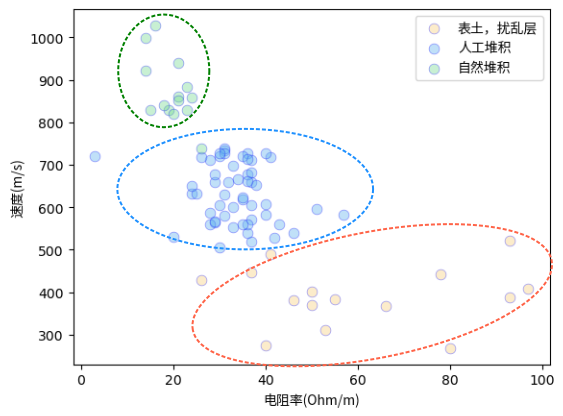
\includegraphics[width=\textwidth]{figure/thesis/output_revised.png}
    \caption{良渚遗址--中心古城区钻孔物性交会图,中心古城区浅层可分为三大类:红色虚线—浅表杂土层、浅蓝色虚线—人工堆积层和绿色虚线—自然堆积层}
    \label{fig:pro_intersection}
\end{figure}

三种地层通过先前的地球物理调查后得到的物性数据如图\ref{fig:pro_intersection}所示,我利用FCM聚类划分了表土层、人工堆积层和自然堆积层。图\ref{fig:pro_intersection}显示三类地层的物性差距较大,如果使用KFCM聚类联合反演应该会有较好的效果。且使用聚类划分后的数据可以利用统计手段得到有效的簇信息,用于后续的KFCM联合反演。

表\ref{tab:center}是通过对物性交会图\ref{fig:pro_intersection}中数据进行统计方法得到的中心,是KCM反演的先验信息;表\ref{tab:borehole}是岩心属性表,不用于先验信息,而是对最后反演的结果进行检验。土芯由洛阳铲采集,并由考古学家分为以下文化层:(1)A层,现代灰色耕地表土层;(2)B层,汉代灰色砂土层(距今约2000年);(3)C层,烧土之上的棕色新石器时代夯土;(4)D层,新石器时代的混合灰和木炭粉的烧土层;(5)E、F层,烧土下方的过渡层和棕色新石器时代夯土。

\begin{table}[h]
\centering
\begin{tabular}{|l|l|l|l|}
\hline
层位 & 自然堆积层 & 人工堆积层 & 杂填土 \\ \hline
电阻率$(\Omega \cdot m)$ & 19.64 & 33.55 & 60.33 \\ \hline
速度$(m/s)$ & 873.35 & 633.70 & 391.93 \\ \hline
\end{tabular}
\caption{中心古城区的先验速度和电阻率数据类簇中心}
\label{tab:center}
\end{table}

\begin{table}[h]
\centering
\begin{tabular}{|l|llll|ll|}
\hline
土壤层 & \multicolumn{4}{l|}{浅表杂土层} & \multicolumn{2}{l|}{人工堆积层} \\ \hline
文化层 & \multicolumn{1}{l|}{A} & \multicolumn{1}{l|}{B} & \multicolumn{1}{l|}{C} & D & \multicolumn{1}{l|}{E} & F \\ \hline
深度(cm) & \multicolumn{1}{l|}{0-30} & \multicolumn{1}{l|}{30-80} & \multicolumn{1}{l|}{80-130} & 130-180 & \multicolumn{1}{l|}{180-280} & 280- \\ \hline
\end{tabular}
\caption{岩芯属性表}
\label{tab:borehole}
\end{table}

\subsection{KFCM聚类联合反演}

在联合反演之前,我们需要确定目标函数的各项系数以及初始模型。结合中央古城的测线所在位置的地质情况和测线长度,最终将反演的模型深度设置为5m,为了能够使最终的反演结果能够显示更精准的纵向层位信息,我们选择反演网格大小为$0.2m\times0.2m$。在进行KFCM联合反演时,我们结合该地区之前得到的钻孔数据和土壤层的层厚,最终将反演的物性类簇数选择为2。在本实验中,我选择的初始模型是线性初始模型,该模型的数值与先验信息相吻合,一共有25层,其中第一层的物理性质(包括速度参数和电阻率等)都略小于杂填土观测到的聚类中心对应的物理性质的值;最后一层的物理性质则略大于人工堆积层所观测到的聚类中心对应的物理性质的值。

至于目标函数的系数,如(\ref{fcmformula})所表示,如果数据和先验信息完整,那么需要确定五组参数:速度数据和电法数据项的权重、震法和电法的正则化项权重和一组耦合系数。我以以下方法确定反演参数:

\begin{itemize}
    \item 利用单独反演的L-曲线法确定每种反演方法的正则化项权重
    \item 进行无耦合的联合反演。如果目标函数收敛,我们就可以选择两者下降速度基本一致的两组权重系数以作为数据项的权重。
    \item 利用L-曲线法,即在保证其他项获取的权重系数比例固定的情况下,计算耦合项和所有数据项的L曲线图。
\end{itemize}

通过上面的步骤,我们可以得到联合反演目标函数的权重。我们首先绘制L-曲线:我选择了从5到500之间不等的多组正则化系数进行单独反演,得到模型误差和数据误差的关系,以此确定一个最合适的正则化系数。本研究根据得到的L-曲线(见图\ref{fig:L_curve})方法得到的速度项的正则化系数是20,得到的电阻率项的正则化系数是20。

\begin{figure}[ht]
    \centering
    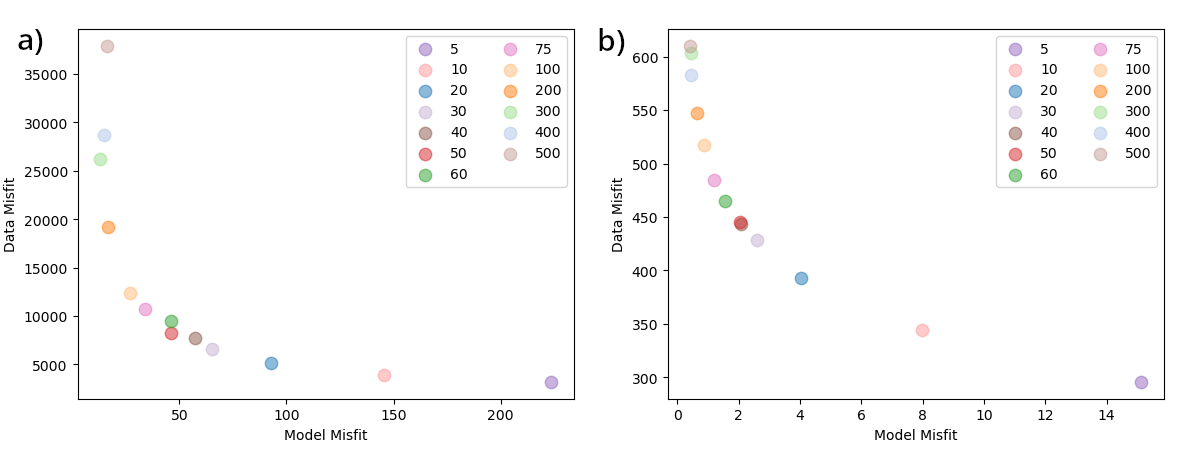
\includegraphics[width=0.9\textwidth]{figure/thesis/L_curve.png}
    \caption{联合反演权重系数决断图。 (a) 良渚遗址的ERT和 (b) 良渚遗址的SRT数据L-曲线图}
    \label{fig:L_curve}
\end{figure}

接下来我确定数据项的系数,我利用确定好的正则化系数进行联合反演。在进行联合反演的过程中,我将耦合项系数设置为1, 保证它不会对数据项的选择造成影响;然后我对两组数据项分别使用了0.1至200不等间隔的数组数据项权重系数进行反演,观察它的RMS值随着迭代步数下降的趋势。如果有一组系数的RMS下降趋势类似,我就选择它来作为反演的数据项系数。根据(图\ref{fig:rms_curve})与使用此数据项得到的反演结果,可以看到不同电阻率数据项的选取,对反演结果迭代速度有较大的影响;而不同的速度数据项则对反演的迭代速度有较小的影响。基于上述结果,我最终决定使用电阻率数据的数据项为2.0,速度数据的数据项为1.0进行下一步的反演。

\begin{figure}[ht]
    \centering
    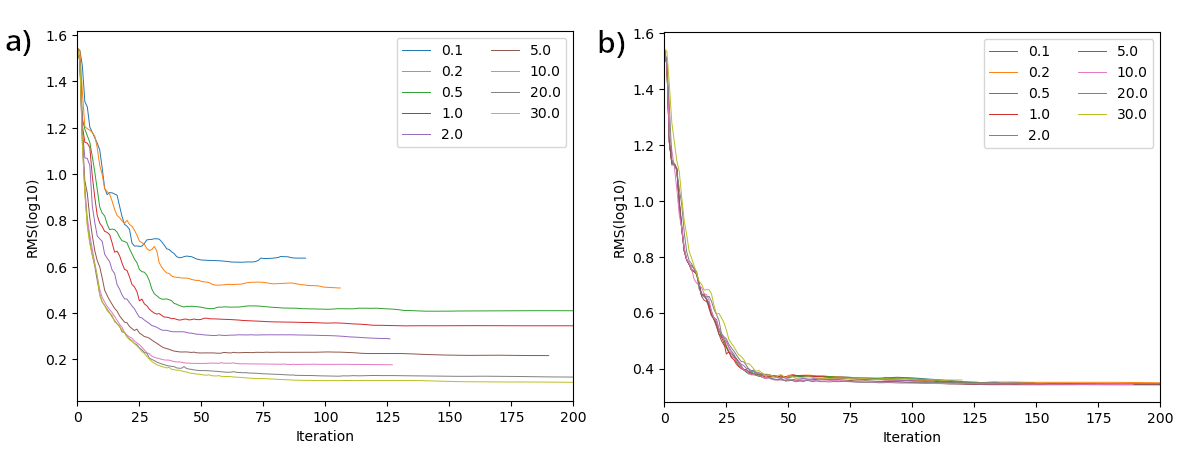
\includegraphics[width=0.9\textwidth]{figure/thesis/rms_curve.png}
    \caption{联合反演权重系数决断图。无耦合项共同反演(a)SRT、(b)ERT的RMS与迭代次数演化图}
    \label{fig:rms_curve}
\end{figure}

最后一步是确定反演的耦合系数,我在L-曲线法的基础上观察结果,挑选最适合的反演的耦合系数。我先以耦合系数项的失配项为X轴,以数据项的失配项为Y轴,得到了联合反演耦合系数决断图。这组L-曲线是为了优化耦合系数项的失配项和数据项的失配项,我们选择两组失配项都较小的对应的耦合系数作为反演的结果。最终综合最后反演结果和L-曲线两者结果,我最终确定耦合系数为1000是最佳的结果。

\begin{figure}[ht]
    \centering
    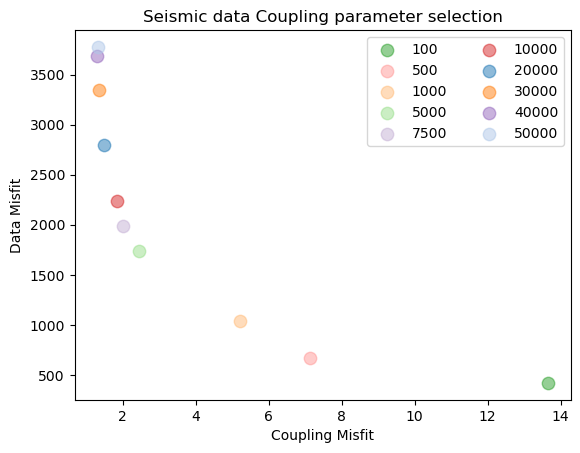
\includegraphics[width=0.8\textwidth]{figure/thesis/coupling.png}
    \caption{联合反演权重系数决断图,良渚遗址进行联合反演的L-曲线图}
    \label{fig:coupling}
\end{figure}

\newpage
\section{结果与分析}
\subsection{单独反演的结果}

展示联合反演的结果之前我先利用相同的数据进行了单独反演,我使用了与联合反演时所用的模型相同的初始模型,但是没有加入先验信息。使用带有约束参数的单独反演得到的结果如下图\ref{fig:ind_inv}所示:
\begin{figure}[ht]
    \centering
    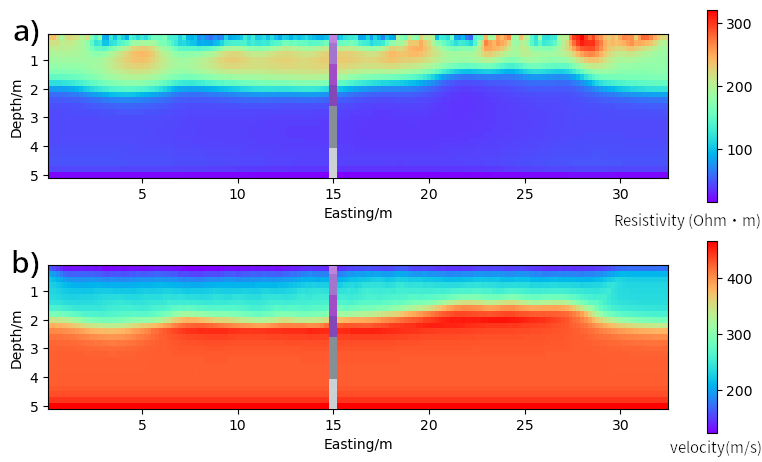
\includegraphics[width=\textwidth]{figure/thesis/individual.png}
    \caption{良渚遗址地下的速度数据和电阻率数据单独反演结果。a)良渚遗址电阻率的单独反演结果,b)良渚遗址速度的单独反演结果;图中色柱是岩性数据,它的数值在\ref{tab:borehole}中}
    \label{fig:ind_inv}
\end{figure}

图\ref{fig:ind_compare}是利用反演预测的数据和初始模型的比较;可以看到,经过两百次左右的迭代,本来的线性初始模型已经可以部分反映出地下介质的状况,且物性分布范围已经收敛,物理参数图已经出现了两个峰值,意味着表土层和人工对基层已经成功地被区分开。但是可以看到电阻率和速度参数的结果均有一定的模糊,部分界面仍然没有很好地区分开来(如速度结果的左边界和右边界两处),且反演结果的具体边界信息与已知钻孔位置吻合效果不好。在物理参数图显示的峰值中,除了层厚较大的人工堆积层外,表土层在物理参数图中反映出来的峰值相对并不明显,所以单独反演的结果相对后文的联合反演来说,区分两层的能力相对较弱。

\begin{figure}[ht]
    \centering
    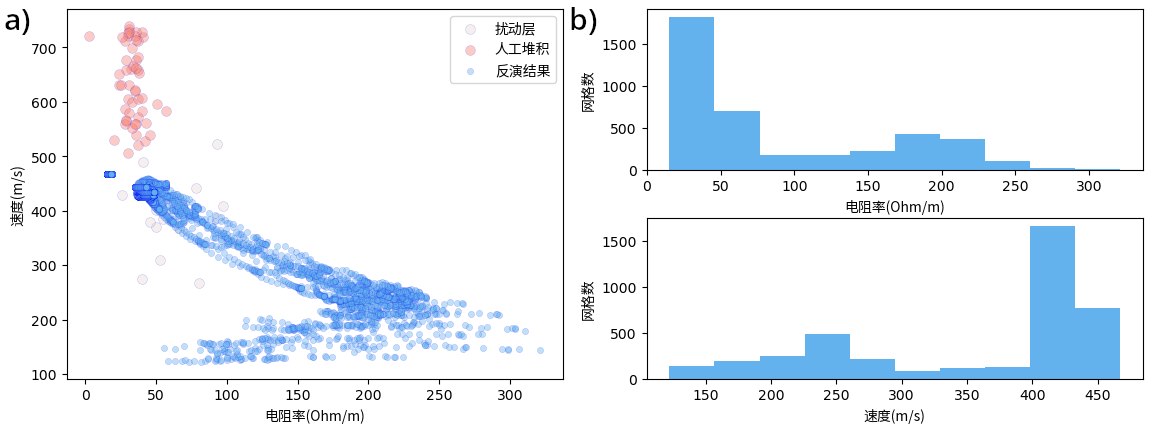
\includegraphics[width=\textwidth]{figure/thesis/res_ind.png}
    \caption{良渚遗址地下的速度数据和电阻率数据单独反演结果与先验信息的对比。a)单独反演的物性交会图,b)物理参数立方图,上图是电阻率参数,下图是速度参数}
    \label{fig:ind_compare}
\end{figure}


\subsection{KFCM联合反演的结果}

使用调整好的系数和初始模型进行反演的结果如\ref{fig:fcm_inv}所示。可以看到它较好地区分了表土层和人工堆积层的界面,并且对于表层的刻画比较清晰。速度结果能够更较为准确的刻画出人工堆积层的上层边界位置,改善了单独反演中对边界刻画较为模糊的缺点。物性交会图也更加地连续,物性参数单元交会图(如\ref{fig:ind_compare}所示)上也出现了两个较为明显的类别峰值。在物性交会图上我们可以看到,由于速度信息相对电阻率信息分布的范围更广,所以在反演模型中,速度的分层界面相对电阻率的分层界面要更为明显,且速度的分层界面中有一层速度约为400m/s的烧土层,这是表土层的下界面。电阻率结果的人工堆积层与现有的钻孔资料吻合得较好,但是,由于该剖面的人工堆积上与烧土层的电阻率相互混杂,导致了聚类联合反演的电阻率结果并不能很好地划分出人工堆积层最上层边界位置。不过好在它们的速度参数直接存在明显的速度差异,因此,我们可以从速度的反演结果上清晰地观察到人工堆积层上边界的位置。


\begin{figure}[ht]
    \centering
    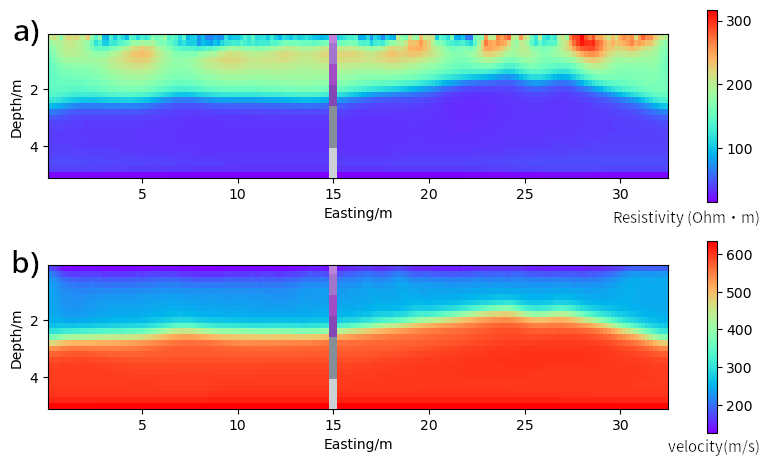
\includegraphics[width=\textwidth]{figure/thesis/fcm_result.png}
    \caption{良渚遗址地下的速度数据和电阻率数据单独反演结果。a)良渚遗址电阻率的KFCM联合反演结果,b)良渚遗址速度数据的KFCM联合反演结果;图中色柱是岩性数据,它的数值在\ref{tab:borehole}中}
    \label{fig:fcm_inv}
\end{figure}

KFCM联合反演交会图能够很好地观察到我们预设的两个类簇,并且由于使用加入了先验的物性数据的引导核模糊C-均值聚类方法(Guided Kernelized Fuzzy C-Means Clustering)使得反演的结果在原先相对精确的模型之上,层位也向正确的观测数据靠近。电阻率结果的人工堆积的F层与钻孔吻合更好,但是该剖面的人工堆积(E)层和烧土层(D)层相混杂,所以该边界并没有被很清晰地刻画出来,但是这两层存在明显的速度差异,因此,从速度的反演结果上我们可以看到到人工堆积层(E层)上边界位置。虽然聚类联合反演能够很好的反演出层间边界位置和物性信息,但是反演的结果似乎会减弱了层间的非均一性,这也许是因为加入的耦合项会试图不断让物性值靠近类簇中心导致的,只要耦合项不为0,该缺点会一直存在。虽然本实验中采取的是单一的耦合项系数,但是我们可以在反演后期不断地降低耦合项权重以图缓解这一问题。

\begin{figure}[ht]
    \centering
    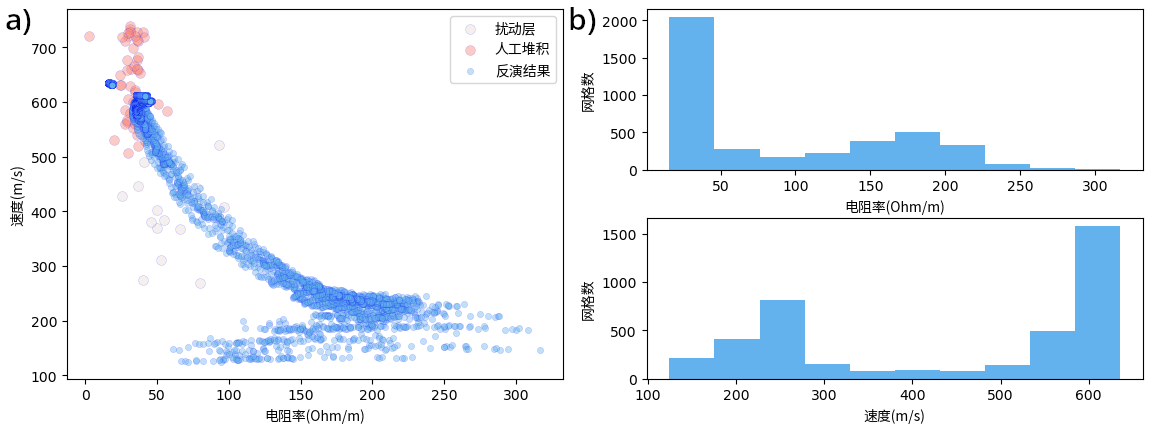
\includegraphics[width=\textwidth]{figure/thesis/res_predict_hist.png}
    \caption{良渚遗址地下的速度数据和电阻率数据KFCM联合反演结果与先验信息的对比。a)KFCM联合反演的物性交会图,b)物理参数立方图,上图是电阻率参数,下图是速度参数}
    \label{fig:fcm_compare}
\end{figure}

\subsection{对结果的分析}

通过对单独反演的结果和KFCM联合反演结果的详细分析,两者的结果都结果均显示出了基本的三层结构。我们可以看到单独反演能够很好的反映出该剖面的大致层位信息,但是部分区域由于数据源单一,所以刻画得相对不如联合反演清晰;而KFCM联合反演交会图能够很好地观察到我们预设的两个类簇(即从先验信息中得到的表土层和人工堆积层)。根据得到的岩芯数据,单独反演的电阻率剖面由于缺少先验数据,得到的层位深度普遍有0.5m左右的偏移;而地震数据则因为精度高且速度变化明显,因此反演的层位与岩芯数据的差距较小。KFCM联合反演(图\ref{fig:fcm_inv}a) b))不仅反映出了地层间的具体层位信息,而且获取了更加接近理论模型的物性信息(图\ref{fig:fcm_compare})。可以看出引导KFCM通过加入人工堆积层物性中心先验信息后,在保留了FCM聚类方法对于结构反演较为精确的特点,还保留了从先验信息中得到的正确层位的信息。

单独反演的电阻率结果虽然在结构上与联合反演的电阻率在结构上结果非常相似,但是由于缺少了额外的速度数据,在表土层的刻画上还是略逊一筹;而缺少的先验信息使得两个电阻率的模型在数值上差异较大:单独反演的表土层深部的电阻率集中在190$\Omega\cdot m$左右,而联合反演的表土层深部的电阻率仅仅大约在150$\Omega\cdot m$左右,再浅一些的部分差异更大。这使得单独反演的结果与实际观测到的数据有较大的差异。

另一个值得一提的部分是不同层位的反演模型的精度。对于同一个反演结果,我们可以看到图\ref{fig:fcm_inv}a)中电阻率层位的数据,很明显表土层的对应情况明显没有人工堆积层的对应情况要好。推测是因为先验信息的数量和质量对引导KFCM的结果有一定的影响。在图\ref{fig:pro_intersection}中我们可以看出人工堆积层的数据相比表土层的数据的点位要多,且人工堆积层在物性交会图中的表现出更强的簇状特征。

总而言之,引导KFCM联合反演,能够更好的刻画边界位置新信息和层间物性值。但是,该方法依赖于大量完整而正确的先验信息。

\newpage
\section{结论与展望}

\subsection{结论}

联合反演对于提高多个物理数据集的反演精度有较大的作用。在复杂的浅地表环境下,结构耦合方法对结构相似性的假设已经不再生效;而基于物性的联合反演方法对于难以获取准确物性关系的环境下不太使用;基于KFCM聚类的联合反演方法有较大的提升,但是如果准确的类簇数和类簇中心信息,仍然会导致结果反常。因此,通过实际实例验证所提方法的有效性,并得到了以下结论:

(1)良渚遗址实验数据都验证了地震走时和直流电阻率数据KFCM或引导KFCM联合反演对于使用单一地球物理数据集的单独反演有着较大的优越性。KFCM聚类联合反演能够解决浅地表团簇状分布模型的问题,同时,如果利用引导KFCM引入先验信息,准确度会进一步提升。

(2)聚类联合反演在地质结构的边界和数据的准确性上明显优于单独反演。在处理物性数据时使用聚类算法分离不同层位的先验信息,可以为后续的联合反演打下坚实基础。

\subsection{展望}

本文提出了电、震的KFCM聚类联合反演方法,并使用良渚遗址的实际案例证明了其有效性,但本文研究工作也存在一些需要进一步探究的问题:

1. 本文使用的KFCM聚类联合反演中所用的FCM算法是针对在物性交会图中呈现类簇状特征的介质属性。如果地层中的介质属性呈现与类簇状不同的形状的话,该算法得到的结果可能不再比单独反演清晰,需要另外开发核函数。

2. 本文使用的介质先验信息虽然较为准确,但是不同层位的先验信息的质量并非完全一致,这导致反演时得到的不同层的反演效果略有差别,后续可以将该方法使用的先验信息做进一步处理以提高联合反演的精度。